%%% -*-LaTeX-*-

\chapter{Definitions}
\label{ch:definitions}

In order to facilitate discussion through this dissertation, we will first establish a common language by defining terms from different areas of mathematics.
%
You may already be familiar with many of these terms, however the goal here is to provide a formal structure and allow us to use certain terms with more precision in order to facilitate later discussion.
%
In some cases, I will be using terms in a context that may differ from other academic works, and so it is important at the outset to be clear what is meant by the terms you will see throughout this document.
%
For example, let me begin with a term that we qualified in Chapter~\ref{ch:introduction}: \emph{data}.

Colloquially, we know data to be some collection of information.
%
However, data can come in many forms, sizes, and structures, so if we are to spend any amount of time talking about techniques that generate, manipulate, and/or analyze data, we also need to be clear what kinds of data.
%
For example, data may be numeric or nominal as in the case of text-based data.
%
With numeric data, a common task is to compute statistical information which cannot be done directly on nominal data.
%
Instead, we may look into building relationships between items in a nominal dataset.
%
Furthermore, data may be time-dependent (temporal) or static in nature.
%
Treating time as a standalone entity rather than as another dimension in the data affords us the opportunity to look at the data in a different light that is not always a sensible paradigm with static data, and so specific methods have been discovered for dealing directly with this type of data.
%
Recall, that for this work, we are focusing on \emph{point cloud} data of \emph{arbitrary dimension} that is defined or can approximated by a \emph{scalar function}.
%
By the end of this chapter, we should have the necessary vocabulary to precisely define what kinds of data this includes.

We shal assume such data can be stored in a tabular format and we will refer to such a table as a dataset where each row represents a different point and the columns represent different dimensions. This leads us to the following set of elementary definitions:

\begin{defn}
  \textbf{Tuple}/\textbf{vector}/\textbf{point} ($\mathbf{x}$) - an ordered collection of real-valued, numeric elements. A tuple will be represented using a bold-faced, lowercase letter.
\end{defn}

\begin{defn}
  \textbf{Dataset} ($\mathbf{X}$) - a finite sequence of tuples, each of the
  same length. We will use a bold-faced, capital letter to denote a full dataset.
\end{defn}

\begin{defn}
  \textbf{Dimension} - either a single element of a tuple or the
  union of all of corresponding elements in all tuples of a dataset.
  The \textbf{dimensionality} of a dataset is the length of any constituent
  tuple.
\end{defn}

An optional subscript may be used when referencing a point to denote its position in $\mathbf{X}$, for example $\mathbf{x_i}$ represents the $i$th entry in the dataset $\mathbf{X}$.
%
When referencing a single element of a point, we will use the convention of an italicized lowercase letter, with either one or two subscripts.
%
For example, $x_{i,j}$ references the $j$th dimension of the $i$th point.
%
In the case, where a point does not define its index, such as $\mathbf{x}$, then $x_j$ represents the $j$th element of the point.

The table or matrix format is a convenient representation, and thus, we can interchangeably use the terms ``row,'' ``entry,'' ``tuple,'' or ``point,'' to describe a horizontal row in the table.
%
The terms ``column,'' ``parameter,'' ``factor,'' and ``dimension'' all describe a vertical column of the data.

%\vspace{10mm}
%\begin{table}[h]
%\centering
%%\captionsetup{justification=centering}
%\begin{tabular}{|l|ccc|r|}
%  \hline
%  $\mathbf{d_0}$ & $\mathbf{d_1}$ & $\ldots$ & $\mathbf{d_{n-1}}$ & $\mathbf{d_n}$\tikzmark{col} \\
%  \hline
%  \hline
%  \tikzmark{row}$x_{0,0}$ & $x_{0,1}$ & $\ldots$ & $x_{0,n-1}$ & $x_{0,n}$ \\
%  \hline
%  $x_{1,0}$ & $x_{1,1}$ & $\ldots$ & $x_{1,n-1}$ & $x_{1,n}$ \\
%  $\vdots$ & $\vdots$ & $\ddots$ & $\vdots$ & $\vdots$ \\
%  $x_{m-1,0}$ & $x_{m-1,1}$ & $\ldots$ & $x_{m-1,n-1}$ & $x_{m-1,n}$ \\
%  \hline
%  $x_{m,0}$ & $x_{m,1}$ & $\ldots$ & $x_{m,n-1}$ & $x_{m,n}$ \\
%  \hline
%\end{tabular}
%\caption[Data viewed as a table]{High-dimensional data can be viewed as a table of
%information organized into rows and columns corresponding to points and dimensions
%of a high-dimensional space, respectively.}
%\label{table:dataTable}
%\end{table}
%\begin{tikzpicture}[remember picture,overlay]
%  \node [above right = 10mm and -41mm] at ({pic cs:col}) (myCol) {\textbf{column/parameter/factor/dimension}};
%  \draw [<-, ultra thick] ([xshift=-10pt, yshift=12pt]{pic cs:col}) to (myCol);
%\end{tikzpicture}
%\begin{tikzpicture}[remember picture,overlay]
%  \node [above left=-3mm and 5mm] at ({pic cs:row}) (myRow) {\textbf{row/entry/tuple/point}};
%  \draw [<-, ultra thick] ([xshift=-8pt, yshift=2pt]{pic cs:row}) to (myRow);
%\end{tikzpicture}
%\vspace{-10mm}

\section{Set Theory}

As we will be discussing collections of data objects and decomposing them into groups or sets, we begin by defining concepts from set theory.
%
\begin{defn}
  \textbf{Set} ($x \in A$) - an unordered collection of finite or infinite objects, $x$.
  %
  A constituent object, $x$, of $A$ is known as a \textbf{member}/\textbf{element}, the relationship being denoted as $x \in A$.
\end{defn}

Numeric sets can be \emph{uncountable} such as the set of all real numbers, $\{x| x \in \mathbb{R}\}$, or \emph{countable} such as the set of all integers, $\{x| x \in \mathbb{Z}\}$ where each item is discrete and isolated.
%
In addition, a set may be \emph{unbounded} as in the above two examples or either \emph{open} or \emph{closed bounded} such as the set $\{x \in \mathbb{R} | x \in [0,1)\}$ which exhibits both characteristics.
%
That is, $0 \le x < 1$, where the lower boundary is closed as it includes the lower bounding value and the upper bound is open.

\begin{defn}
  \textbf{Cardinality} ($|A|$) - The number of elements in a set.
\end{defn}

\begin{defn}
  \textbf{Empty set}/\textbf{null set} ($\emptyset$) - a set containing no members.
\end{defn}

\begin{defn}
  \textbf{subset} ($C \subseteq A$) - If every element of $C$ exists in $A$, then $C$ is a subset of $A$.
  %
  Furthermore, $C$ is a \textbf{proper subset} ($C \subset A$) when $C \neq A$.
  %
  In other words, when $A$ contains at least one member that is not in $C$.
\end{defn}

The following operators apply to example sets $A$ and $B$:

\begin{defn}
  \textbf{Union} ($A \cup B$) - The set of all elements in $A$ or $B$: $A \cup B = \{x| x \in A$ or $x \in B\}$.
\end{defn}

\begin{defn}
  \textbf{Intersection} ($A \cap B$) - The set of all elements in $A$ and $B$: $A \cap B = \{x| x \in A$ and $x \in B\}$.
\end{defn}

\begin{defn}
  \textbf{Difference} ($A$ $\backslash$ $B$) - The set of all elements in $A$ and not in $B$: $A$ $\backslash$ $B = \{x| x \in A$ and $x \notin B\}$.
  %
  Note that this operation is not commutative as $A$ $\backslash$ $B = B$ $\backslash$ $A \Rightarrow A = B$.
\end{defn}

\begin{defn}
  \textbf{Partition} - A collection of subsets of $A$ such that every element of $A$ exists in one and only one of the subsets.
  %
  That is, the intersection of any subsets making up a partition will be empty: $C \cap D = \emptyset$, if $C$ and $D$ are part of the same partition.
\end{defn}

\section{Calculus}

Under certain contexts throughout this document, it will be useful to separate a dataset into independent and dependent dimensions, also referred to as inputs and outputs, or variables and responses, respectively.
%
In these cases, the same notations apply except that the letter $x$ will be used to denote input(s) and $y$ will denote output(s).
%
Such datasets exist when $\mathbf{y}$ (either a scalar or vector) can be represented as a function of a tuple of inputs $\mathbf{x}$, $\mathbf{y}=f(\mathbf{x})$.
%
A function, $f$, fulfills the requirement that any input $\mathbf{x}$ be associated to at most one output, or set of outputs in the case where $\mathbf{y}$ is defined by multiple dimensions.
%
Below is the formal definition of a function as it relates to the earlier described set theory:

\begin{defn}
  \textbf{Function}/\textbf{map} ($f : X \rightarrow Y$) - Assigns each
  element in $X$ ($x \in X$) to exactly one element in $Y$ ($y \in Y$).
  In terms of sets, the notation $f : X \rightarrow Y$ is read as $f$
  maps $X$ into $Y$, and in terms of elements $f(x)=y$ is read as $f$ maps $x$
  to $y$.
  In this example, $X$ is the \textbf{domain} of $f$ and $Y$ is the
  \textbf{codomain}, or \textbf{range}, of $f$. Also, $y$ is the \textbf{image},
  of $x$ under $f$.
\end{defn}

Relevant functional properties are described below:

\begin{defn}
  \textbf{Injection}/\textbf{One-to-one function} - Every point in the domain
  maps to a distinct element in the codomain. Symbolically, the function
  $f:X\rightarrow Y$ is injective if $\forall a,b\in X,f(a)=f(b)\Rightarrow a=b$
\end{defn}

\begin{defn}
  \textbf{Surjection}/\textbf{Onto function} - Every point in the codomain is
  associated to some point in the domain. Symbolically, the function
  $f:X \rightarrow Y$ is surjective if $\forall y \in Y,\exists x \in X,f(x)=y$
\end{defn}

\begin{defn}
  \textbf{Bijection} - A function that is both injective and surjective. As a
  result, a bijective function $f: X \rightarrow Y$ also has an inverse mapping
  $f^{-1} : Y \rightarrow X$.
\end{defn}

\begin{defn}
\textbf{Derivative}$\mathbf{(\frac{df}{dx})}$ - Given a function $f(x)$ defined
 as $f : \mathbb{R} \rightarrow \mathbb{R}$,
 $\frac{df}{dx} = \lim_{h\rightarrow 0}\frac{f(x+h)-f(x)}{h}$.
 The generalization to an $n$-dimensional domain adds the notion of a
 \textbf{partial derivative} ($\frac{\partial f}{\partial x_0}$), where all but
 one parameter are held constant, thus: $\frac{df}{dx_i} =
 \lim_{h\rightarrow 0}\frac{f(x_1,...,x_i+h,...x_n)-f(x_1,...,x_i,...,x_n)}{h}$.
 The derivative is itself a function, and thus the $n^{th}$-derivative is
 achieved by successively applying the derivative operation and is deonted
 as $\frac{d^nf}{dx^n}$. For the multidimensional case, partials of partials can
 be applied along arbitrary dimensions to achieve mixed partials.
\end{defn}

\begin{defn}
  \textbf{Gradient}$\mathbf{(\nabla f(\mathbf{x}))}$ - Given $f : \mathbb{R}^n \rightarrow \mathbb{R}$, then $\nabla f = \left(\frac{\partial f}{\partial
  x_1},...,\frac{\partial f}{\partial x_{n}}\right)$
  The gradient of a function where the domain is scalar is equivalent to the
  derivative.
\end{defn}

\begin{defn}
  $\mathbf{C^n}$\textbf{Continuity} - $f : A \rightarrow \mathbb{R}^d$ is
  continuous of order $n$ if all orders of differentiation up to $n$ exist and
  are continuously defined on the domain $A$.
\end{defn}

\begin{defn}
  \textbf{Smooth} - A $\mathbf{C^\infty}$ function. Thus, all orders of
  differentiation of a function exist and are continuous on the domain $A$.
\end{defn}

\begin{defn}
  \textbf{Critical point} - Any domain location $\mathbf{x}$ where $\nabla
  f(\mathbf{x}) = \mathbf{0}$. All other locations are considered
  \textbf{regular}.
\end{defn}

\begin{defn}
  \textbf{Hessian} ($H_f(p)$) - A square $d\times d$ matrix achieved by evaluating
  all of the second order partials of $f : \mathbb{R}^d \rightarrow \mathbb{R}$ at
  the domain location $\mathbf{p}$:

  $H_f(p) =
  \begin{bmatrix}
    \frac{\partial^2f}{\partial x_1^2}(\mathbf{p}) & & \ldots & & \frac{\partial^2f}{\partial x_1\partial x_d}(\mathbf{p}) \\
     & \ddots &  &  & \\
    \vdots &  & \frac{\partial^2f}{\partial x_i\partial x_j}(\mathbf{p}) &  & \vdots \\
     & &  & \ddots & \\
    \frac{\partial^2f}{\partial x_d\partial x_1}(\mathbf{p}) & & \ldots & & \frac{\partial^2f}{\partial x_d^2}(\mathbf{p}) \\
  \end{bmatrix}$
\end{defn}

\begin{defn}
  \textbf{Degenerate critical point} - A critical point, $\mathbf{p}$, with a
  singular Hessian matrix: $det(H_f(\mathbf{p})) = 0$.
\end{defn}

\begin{defn}
 \textbf{Level set}/\textbf{contour}/\textbf{iso-contour}/\textbf{iso-surface} -
 The collection of domain locations which under a given function ($f : A
 \rightarrow \mathbb{R}$) map to the same constant $c$: $\{\mathbf{x} \in A |
 f(\mathbf{x}) = c\}$.
\end{defn}

\section{Topology}

Though the name of a field of study, there is also a technical definition attached to the word topology that can be formalized through set theory:

\begin{defn}
  \textbf{Topology} - a set $A$ along with a collection of its subsets,
  $\mathcal{T}$, where the subsets of $\mathcal{T}$ satisfy three conditions:

  \begin{enumerate}
  \item $A \in \mathcal{T}$ and $\emptyset \in \mathcal{T}$
  \item If $A_1,A_2 \in T$, then $A_1 \cap A_2 \in \mathcal{T}$
  \item If $\{A_j|j\in J\} \subseteq \mathcal{T}$, then $\cup_{j\in J} A_j \in \mathcal{T}$
  \end{enumerate}
\end{defn}

\begin{defn}
  \textbf{Open set} - Given the topology above $\mathcal{T}$, any set $S$ such
  that $S \in \mathcal{T}$.
\end{defn}

\begin{defn}
  \textbf{Closed set} - Given the topology $\mathcal{T}$ and the open set $S$
  given above, any set $U$ such that $U = A$ $\backslash$ $S$.
\end{defn}

In the abstract sense, this definition is precise, however somewhat unsatisfying.
%
When we restrict our topology to metric spaces, the intuition is that open/closed sets are $n$-dimensional generalizations of an open and closed interval in a 1-dimensional space, respectively.

\begin{defn}
  \textbf{Topological space} - The pair $(A,\mathcal{T}) = \mathbb{A}$ given in
  the defintion of a topology above.
\end{defn}

\begin{defn}
  \textbf{Interior} ($A^{\circ}$) - the union of all open sets
  contained in $A$. Alternatively, it is the maximal open set of $A$.
\end{defn}
\begin{defn}
  \textbf{Closure} ($A^{-}$) - the intersection of all closed sets containing
  $A^{-}$. The closure represents the minimal closed set of $\mathcal{T}$ that
  contains $A$.
\end{defn}
\begin{defn}
  \textbf{Boundary} ($\delta A$) - the closure without the interior:
  $\delta A = A^{-} \backslash A^{\circ}$.
\end{defn}

\begin{defn}
  \textbf{Neighborhood} of $C$ ($\mathcal{N}_C$) - Given a topological space
  $\mathbb{A}=(A,\mathcal{T})$ and $C \subseteq A$, any subset of $A$ containing
  an open set of $\mathbb{A}$ and $C$.
\end{defn}

\begin{defn}
  \textbf{Neighborhood basis} - A set of neighborhoods of $C$,
  from the previous definition, denoted $\mathcal{B}$, where for each
  neighborhood $N$ of $C$, there exists a subset, $M$, in $\mathcal{B}$ such
  that $M \subseteq N$.
  $\{\forall N \in \mathcal{N}_C, \exists M \in \mathcal{B} | M \subseteq N\}$
\end{defn}

\begin{defn}
  \textbf{Isolated point} - $\mathbf{p} \in A$ is an isolated point of a
  subset $C$ ($C \subseteq A$) if $\mathbf{p} \in C$ and there exists a
  neighborhood of $x$ containing no other points of $C$.
\end{defn}

\begin{defn}
  \textbf{Induced/Relative topology} - Given a topological space
  $\mathbb{A}=(A,\mathcal{T})$ and $C \subseteq A$,
  the \textbf{induced}/\textbf{relative} topology is defined as
  $\mathcal{T}_C = \{C \cap S | S \in \mathcal{T}\}$. $C$ is a
  \textbf{topological subspace} of $\mathbb{A}$.
\end{defn}

\begin{defn}
  \textbf{Metric} - A function, $d: A \times A \rightarrow \mathbb{R}$,
  satisfying four conditions:
  \begin{enumerate}
  \item Positivity: $\forall x,y \in S, d(x,y) \ge 0$
  \item Non-Degeneracy: $d(x,y)=0 \Rightarrow x=y$
  \item Symmetry: $\forall x,y \in S, d(x,y) = d(y,x)$
  \item Triangle Inequality: $\forall x,y,z \in S, d(x,y) + d(y,z) \ge d(x,z)$
  \end{enumerate}
\end{defn}
\begin{defn}
  \textbf{Open ball} ($B(x,r)$) - Defined by a particular metric $d$, to be
  every element closer than $r$ to the element $x$: $B(x,r) = \{y| d(x,y) < r\}$.
\end{defn}
\begin{defn}
  \textbf{Metric space} - A set with a metric function.
\end{defn}

Within a metric space, the abstract concepts of topology become more concrete and easier to understand.
%
For instance, open balls become the realization of the notion of open set, and the boundary of the open ball is given by $\{y| d(x,y) = r\}$, and thus the closure of an open set is given by $\{y| d(x,y) \leq r\}$.
%
A neighborhood of an element can then be thought of as an open ball.
%
A few examples of such are given in Euclidean space below, but first we define the Euclidean space formally:

\begin{defn}
  \textbf{$n$-dimensional Euclidean space} ($\mathbb{E}^n$) - The combination of
  the set defined by the n-dimensional real space, $\mathbb{R}^n$ and the
  \textbf{Euclidean metric}: d(x,y) = $\sqrt{\sum_i=0^n(x_i-y_i)^2}$.
\end{defn}

\begin{figure}[t]
  \centering
  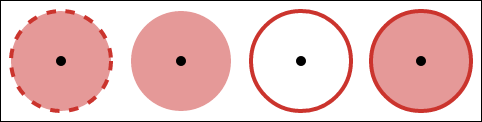
\includegraphics[width=.75\textwidth]{figs/chap2/openSet}
  \caption[Open ball as an example of an open set]{From left to right: An open
  ball as an example of an open set around point
  $\mathbf{p}$ in $\mathbb{E}^2$, the interior of the open set, the boundary of
  the open set, and the closure of the open set.}
  \label{fig:graphs}
\end{figure}

% \nb{Insert example of an open set, interior, closure, and boundary of a circle,
% topological subspace, neighborhood}

\begin{defn}
  \textbf{$n$-dimensional Euclidean half-space} - A subset of $\mathbb{E}^n$
  partitioned by an $(n-1)$-dimensional hyperplane and is denoted
  as $\mathbb{H}^n$.
\end{defn}

\begin{defn}
  \textbf{Homeomorphism} - A continuous, bijective function, from one
  topological space $\mathbb{A}$ to another $\mathbb{B}$ ($f :\mathbb{A}
  \rightarrow \mathbb{B}$) whose inverse ($f^{-1}: \mathbb{B}
  \rightarrow \mathbb{A}$), is also continuous.
  $\mathbb{A}$ is said to be homeomorphic to $\mathbb{B}$.
\end{defn}

% \begin{defn}
%   \textbf{Equivalence relation} ($a \sim b$) - A set, $R$,
%   $R \subseteq A \times A$, defines a relationship among elements of a set $A$
%   such that $\{(a,b) \in R| a,b \in A \}$, also written
%   $a R b$, or $a \sim b$ denoting $a$ and $b$ are equivalent or related according
%   to the relation, $R$. Such relationships satistfy the following three
%   properties:

%   \begin{itemize}
%   \item Reflexive: $a \sim a, \forall a \in A$
%   \item Symmetric: $a \sim b \Rightarrow b \sim a, a,b \in A$
%   \item Transitive: $a \sim b$ and $b \sim c \Rightarrow a \sim c, a,b,c \in A$
%   \end{itemize}

%   All points equivalently related under $R$ taken together form an
%   \textbf{equivalence class}.
% \end{defn}
\subsection{Manifolds}

As we discuss topological spaces, it is also important to define a topological manifold.
%
The formal definition implies some terminology from the field of algebraic topology, so first let us informally define what is meant by a manifold.
%
An $n$-manifold (without boundary), $\mathcal{M}$, is a space that locally resembles $\mathbb{R}^n$.
%
That is, given any point in the manifold, its neighborhood of points lying on the manifold maps to a continuous space in $n$-dimensions.
%
This implies a manifold spans a continuous, unbounded space since no point has neighbors on just one ``side'' of the space.
%
For example, consider a line and a circle, both 1-manifolds.
%
In each case, one can define a forward and backward neighbor at any point.
%
The difference being that the circle case has a finite subcover, a finite number of open sets can be used to cover the entire space, making it a \emph{compact} manifold, whereas the line is \emph{non-compact}.
%
At times, we will discuss a \emph{manifold with boundary} where this property does not hold.
%
That is, in the 1-manifold case there may be points where only a forward or backward neighbor is defined, but not both, such as the case of a line segment or a ray.
%
The boundary encompassing a $n$-manifold with boundary is itself an $n-1$-manifold without boundary.
%
An $n$-manifold is a space that is locally \emph{homeomorphic} to the $n$-dimensional real space, $\mathbb{R}^n$, but the manifold itself, is not necessarily homeomorphic to $\mathbb{R}^n$.
%
To put it in the language, we have thus far formally introduced:

\begin{defn}
  \textbf{n-manifold} - a topological space such that every point in the
  space has a neighborhood that is homeomorphic to the $n$-dimensional Euclidean
  space.
\end{defn}

A manifold can be described using charts:

\begin{defn}
  \textbf{Chart} at $a \in \mathbb{A}$ - a homeomorphism mapping a
  neighbhorhood of $a$, $N_a$ to an open set in $\mathbb{R}^n$. Symbolically,
  a chart can be denoted as an ordered pair: $(N_a,f)$, where $f: N_a
  \rightarrow \mathbb{R}^n$ and $n$ is the dimension of the chart.
\end{defn}

\begin{defn}
  \textbf{Atlas} - a collection of charts $\{(N_a,f_a)\}$ defined on a
  topological space $\mathbb{A}$ such that $\cup N_a = \mathbb{A}$.
\end{defn}

\begin{defn}
  \textbf{Hausdorff space} - A topological space where distinct points can
  be identified by disjoint neighborhoods: $\{\forall x,y \in \mathbb{A},
  \exists N_x,N_y | x \in N_x, y \in N_y, x \neq y, N_x \cap N_y = \emptyset\}$.
\end{defn}
\begin{defn}
  \textbf{Separable} topological space - A topological space with a countable
  basis of neighborhoods.
\end{defn}
\begin{defn}
  \textbf{$d$-manifold with boundary} - a manifold such that every point in
  it is homeomorphic to either $\mathbb{R}^d$ or $\mathbb{H}^d$ and the boundary
  is the set of all points with neighborhoods homeomorphic to $\mathbb{H}^d$.
\end{defn}
\begin{defn}
  \textbf{Cover} of set $A$ - a collection of sets whose union contains $A$
  as a subset. A covering is \textbf{open} if it consists of open sets. A
  \textbf{subcovering} of a covering is a subset that is still a covering of the
  original set.
\end{defn}

\begin{defn}
  \textbf{Compact set} - A set where every open cover contains a finite
  subcovering.
\end{defn}

\begin{defn}
  \textbf{Embedding} - a map $f : X \rightarrow Y$ that is a homeomorphism onto
  its image, $f(X)$.
\end{defn}

\subsection{Graphs and Complexes}

As we move from the abstract concepts of topology to the concrete, it will be useful to borrow some terminology from graph theory and geometry.

\begin{defn}
  \textbf{Graph} ($G$) - An ordered pair $(V(G),E(G))$ consisting of a set of
  \textbf{vertices}, $V(G)$, and a set of edges, $E(G)$, combined with an
  \textbf{incidence function}, $\psi_G : E(G) \rightarrow V(G) \times V(G)$.
  That is, a graph consists of a set of vertices and edges connecting those
  vertices. A \textbf{subgraph}, $H = (V(H),E(H))$, of $G$ is defined such that
  $V(H) \subseteq V(G)$ and $E(H) \subseteq E(G)$. $G$ is also the
  \textbf{supergraph} of $H$.
\end{defn}

\begin{defn}
  \textbf{Graph neighbors} - $\{v_1,v_2 \in V(G) | \exists e \psi_G(e) =
  (v_1,v_2) or \psi_G(e) = (v_2,v_1) \}$. Two graph vertices $v_1$ and $v_2$ are
  neighbors if there exists an edge $e$ associating them.
\end{defn}

\begin{defn}
  \textbf{Directed graph} - A graph where the order of the tuple defined by
  $\psi_G(e)$ is respected. If the order of edge tuples does not matter, the
  graph is considered \textbf{undirected}.
\end{defn}

\begin{defn}
  \textbf{Parallel edge} - $\{e_1,e_2 \in E(G) | if \psi_G(e_1) = (v_1,v_2),
  v_1,v_2 \in V(G), then \psi_G(e_2) = (v_1,v_2) or \psi_G(e_2) = (v_2,v_1) \}$
\end{defn}

\begin{defn}
  \textbf{Loop} - $\{e_1 \in E(G) | \psi_G(e_1) = (v_1,v_1), v_1 \in V(G)$.
\end{defn}

\begin{defn}
  \textbf{Simple graph} - A graph with no parallel edges or loops.
\end{defn}

\begin{defn}
  \textbf{Complete graph} - $\{G | \forall v_1,v_2 \in V(G), \exists e\in E(G)
  s.t. \psi_G(e) = (v_1,v_2) or \psi_G(e) = (v_2,v_1)\}$
\end{defn}

\begin{defn}
  \textbf{Path} - A simple graph whose vertices can be arranged into a sequence
  such that the adjacency in the sequence implies connectivity, and
  non-adjacency implies the vertices are not connected in the graph.
\end{defn}

\begin{defn}
  \textbf{Cycle} - A path where the first and last vertices are also adjacent.
\end{defn}

\begin{defn}
  \textbf{Star} - The union of a vertex, all edges emanating from it, and its
  neighbors.
\end{defn}

\begin{defn}
\textbf{bipartite graph} - A graph whose vertices can be partitioned into two sets such that all edges connect a vertex from one partition/equivalence class to a vertex in the other partition/equivalence class.
\end{defn}

\begin{defn}
  \textbf{Connected component} - A subgraph where a path exists connecting
  any two vertices in the subgraph and contains no additional vertices of the
  supergraph.
\end{defn}

\begin{defn}
  \textbf{Convex set} - In Euclidean space, a set such that for every pair of
  points in the set, there exists a straight line segment that is entirely
  inside the set.
\end{defn}

\begin{defn}
  \textbf{Convex hull} of a set - The smallest convex set containing a set of
  points.
\end{defn}

\begin{defn}
  \textbf{$n$-Simplex} - A bipartite graph of $n+1$ vertices in $n$-dimensions
   (plus all \emph{faces} enclosed by cycles of edges).
  Alternatively, it is the convex hull of $n+1$ vertices in $n$-dimension.
\end{defn}

\begin{defn}
  \textbf{Face/cell} - Any simplex that forms a subset of a $k$-simplex.
  The $k$-simplex is called the \textbf{co-face} of any of its faces.
\end{defn}

\begin{defn}
  \textbf{Simplicial Complex} - A set of simplices, $K$ such that any face of
  a simplex in $K$ is itself in $K$, and the intersection of any two simplices
  is either $\emptyset$ or a face of both simplices.
\end{defn}

\begin{defn}
  \textbf{Triangulation} - A simplicial complex, $K$ defined on a topological
  space, $\mathbb{A}$, such that $K \sim \mathbb{A}$
\end{defn}

% \section{Information Theory}
